\documentclass{beamer}
\usepackage[dutch]{babel}
\usepackage{calc}
\usepackage[absolute,overlay]{textpos}
\usepackage{amsmath}
\usepackage{amsthm}
\usepackage{graphicx}
\usepackage{tikz}
\usetikzlibrary{decorations.pathreplacing}
\mode<presentation>{\usetheme{tud}}

\title[NedTrain Planner]{NedTrain Planner}
%\subtitle
\institute[TU Delft]{Construeren van Flexibele Roosters}
\author{Chris Bakker, Anton Bouter, Martijn den Hoedt}
\date{2 juli 2014}

\theoremstyle{definition}
\newtheorem{definitie}{Definitie}[section]

% Insert frame before each subsection (requires 2 latex runs)
\AtBeginSubsection[] {
	\begin{frame}<beamer>\frametitle{\titleSubsec}
		\tableofcontents[currentsection,currentsubsection]  % Generation of the Table of Contents
	\end{frame}
}
% Define the title of each inserted pre-subsection frame
\newcommand*\titleSubsec{Next Subsection}
% Define the title of the "Table of Contents" frame
\newcommand*\titleTOC{Outline}

% define a symbol which can be removed if you don't need it
\newcommand{\field}[1]{\mathbb{#1}}
\newcommand{\Zset}{\field{Z}}

\tikzset{
  invisible/.style={opacity=0},
  visible on/.style={alt={#1{}{invisible}}},
  alt/.code args={<#1>#2#3}{%
    \alt<#1>{\pgfkeysalso{#2}}{\pgfkeysalso{#3}} % \pgfkeysalso doesn't change the path
  },
}

\definecolor{darkyellow}{rgb}{0.7, 0.7, 0}
\definecolor{lightyellow}{rgb}{1.0, 1.0, 0}
\definecolor{darkgreen}{rgb}{0, 0.5, 0}
\definecolor{lightgreen}{rgb}{0, 0.7, 0}
\definecolor{darkcyan}{rgb}{0, 0.7, 0.7}
\definecolor{lightcyan}{rgb}{0, 1.0, 1.0}

\begin{document}

{
% remove the next line if you don't want a background image
\usebackgroundtemplate{\includegraphics[width=\paperwidth,height=\paperheight]{images/background-titlepage.jpg}}%
\setbeamertemplate{footline}{\usebeamertemplate*{minimal footline}}
\frame{\titlepage}
}

\begin{frame}\frametitle{Inhoud}
    \begin{itemize}
        \item Opdrachtgevers
        \item Opdrachtomschrijving
        \begin{itemize}
        	\item Beschrijving Roosters
        	\item Voorbeeld Demo
        	\item Eisen van de Opdrachtgever
        \end{itemize}
        \item Aanpak en Hulpmiddelen
        \item Flexibiliteit
        \item Linear Programming
        \item Chaining Algoritme
        \item Andere Features
        \item Eind Demo
        \item Vragen
    \end{itemize}
\end{frame}

\begin{frame}\frametitle{Opdrachtgevers}
\begin{columns}[T] % align columns
    \begin{column}{.55\textwidth}
        \begin{itemize}
            \item NedTrain 
            \begin{itemize}
                \item Nederlandse Spoorwegen
                \item $250$ treinen op $30$+ locaties
                \item $3500$ werknemers 24/7 
                \item ir. Bob Huisman
            \end{itemize}
        \end{itemize}
        \vspace{1.8cm}
        \begin{itemize}
            \item TU Delft
            \begin{itemize}
                \item Algoritmiek groep
                \item prof. dr. Cees Witteveen
            \end{itemize}  
        \end{itemize}
    \end{column}%
    \begin{column}{.45\textwidth}
        \includegraphics[width=4.5cm]{images/logo-nedtrain.jpg}
        \vspace{1cm}
        \includegraphics[width=5cm]{images/tudelft_logo.pdf}
    \end{column}%
\end{columns}
\end{frame}


\begin{frame}\frametitle{Hoe ziet een rooster eruit?}
    \begin{itemize}
        \item Activiteiten
        \begin{itemize}
            \item Stoelen vervangen
            \item Grafiti verwijderen      
        \end{itemize}
        \item Resources
        \begin{itemize}
            \item Monteurs
            \item Schoonmakers
            \item Werkplaatsen
        \end{itemize}
        \item Constraints
        \begin{itemize}
            \item Deadlines
            \item Stoelen vervangen en daarna de trein schoonmaken      
        \end{itemize}
    \end{itemize}
\end{frame}

\begin{frame}\frametitle{NedTrain Planner}
    
\end{frame}

\begin{frame}\frametitle{Opdrachtomschrijving}
	\begin{itemize}
		\item Functionele eisen
		\begin{itemize}
			\item De capaciteit van de resources mag niet overschreden worden bij het verschuiven van activiteiten
			\item De flexibiliteit van een rooster moet berekend worden
			\item De flexibiliteit van een rooster moet weergegeven en geëvalueerd kunnen worden
		\end{itemize}
		\item Niet-Functionele eisen
		\begin{itemize}
			\item De applicatie moet beschikbaar worden gemaakt voor Windows 7
			\item De applicatie moet makkelijk overdraagbaar zijn voor een volgend project
		\end{itemize}
	\end{itemize}
\end{frame}
\begin{frame}\frametitle{Aanpak en Hulpmiddelen}
	\begin{itemize}
	
	\end{itemize}
\end{frame}
\begin{frame}\frametitle{Flexibiliteit (1)}
    \begin{itemize}
        \item Hoe wordt flexibiliteit gemeten?
        \begin{itemize}
            \item<4-> Voor \'e\'en taak: $flex_t = t^+ - t^-$
        \end{itemize}
    \end{itemize}

    \newcommand{\widthpic}{100mm}
    \newcommand{\heightpic}{10mm}
    \newcommand{\offset}{2mm}
    \begin{tikzpicture}
        \coordinate (A) at (0, \heightpic /2);
        \coordinate (B) at (\widthpic, \heightpic /2);
        \coordinate (A1) at (0, 0);
        \coordinate (A2) at (0, \heightpic);
        \coordinate (B1) at (\widthpic, 0);
        \coordinate (B2) at (\widthpic, \heightpic);

        \draw [very thick] (A) -- (B);

        \filldraw[very thick, draw=darkgreen,fill=lightgreen, visible on=<1>] (10mm, \offset) rectangle (35mm, 8mm);
        \filldraw[very thick, draw=darkgreen,fill=lightgreen, visible on=<2>] (0mm, \offset) rectangle (25mm, 8mm);
        \filldraw[very thick, draw=darkgreen,fill=lightgreen, visible on=<3->] (75mm, \offset) rectangle (100mm, 8mm);

        \node[visible on=<2->] at (0mm,-3mm) {$t^-$};
        \node[visible on=<3->] at (75mm,-3mm) {$t^+$};

        \draw [very thick] (A1) -- (A2);
        \draw [very thick] (B1) -- (B2);
    \end{tikzpicture}
\end{frame}

\begin{frame}\frametitle{Flexibiliteit (2)}
    \begin{itemize}
        \item Hoe wordt flexibiliteit gemeten?
        \begin{itemize}
            \item Voor \'e\'en taak: $flex_t = t^+ - t^-$
            \item Voor hele schema: $flex_{totaal} = \sum_{t \in T}(t^+ - t^-)$    
            \item<2-> Voorrangsrelatie: $a \prec b$
        \end{itemize}
    \end{itemize}

    \newcommand{\widthpic}{100mm}
    \newcommand{\offset}{2mm}
    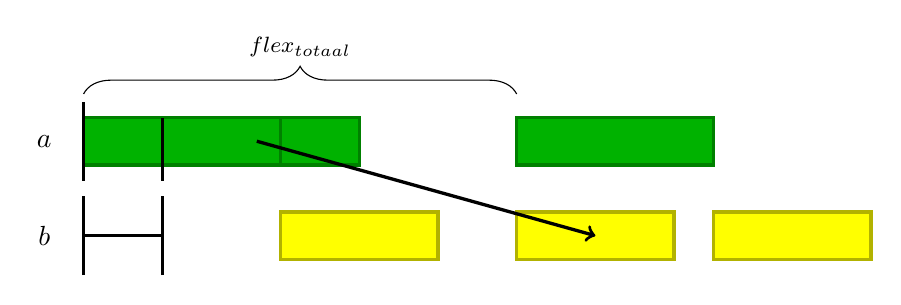
\begin{tikzpicture}
        \coordinate (A) at (0, 17mm);
        \coordinate (B) at (\widthpic, 17mm);
        \coordinate (A1) at (0, 12mm);
        \coordinate (A2) at (0, 22mm);
        \coordinate (B1) at (\widthpic, 12mm);
        \coordinate (B2) at (\widthpic, 20mm);

        \coordinate (C) at (0, 5mm);
        \coordinate (D) at (\widthpic, 5mm);
        \coordinate (C1) at (0, 0mm);
        \coordinate (C2) at (0, 10mm);
        \coordinate (D1) at (\widthpic, 0mm);
        \coordinate (D2) at (\widthpic, 10mm);

        \draw [very thick] (A) -- (B);
        \draw [very thick] (C) -- (D);

        \node at (-5mm,17mm) {$a$};
        \node at (-5mm,5mm) {$b$};

        % ergens in het midden
        \filldraw[very thick, draw=darkgreen,fill=lightgreen, visible on=<1-2>] (10mm, 14mm) rectangle (35mm, 20mm);
        \filldraw[very thick, draw=darkyellow,fill=lightyellow, visible on=<1-2>] (55mm, 2mm) rectangle (75mm, 8mm);

        % aan het begin
        \filldraw[very thick, draw=darkgreen,fill=lightgreen, visible on=<3>] (0mm, 14mm) rectangle (25mm, 20mm);
        \filldraw[very thick, draw=darkyellow,fill=lightyellow, visible on=<3>] (25mm, 2mm) rectangle (45mm, 8mm);

        % aan het einde
        \filldraw[very thick, draw=darkgreen,fill=lightgreen, visible on=<4->] (55mm, 14mm) rectangle (80mm, 20mm);
        \filldraw[very thick, draw=darkyellow,fill=lightyellow, visible on=<4->] (80mm, 2mm) rectangle (100mm, 8mm);
        
        % curly bracket
        \draw [decorate,decoration={brace,amplitude=10pt}, visible on=<5>]
        (0mm,23mm) -- (55mm,23mm) node [black,midway, yshift=6mm] 
        {\footnotesize $flex_{totaal}$};

        \draw [very thick] (A1) -- (A2);
        \draw [very thick] (B1) -- (B2);
        \draw [very thick] (C1) -- (C2);
        \draw [very thick] (D1) -- (D2);

        \draw [very thick, ->, visible on=<2>] (22mm, 17mm) -- (65mm, 5mm);
    \end{tikzpicture}
\end{frame}

\begin{frame}\frametitle{Flexibiliteit (3)}
    \begin{itemize}
        \item Voor hele schema: $flex_{totaal} = \sum_{t \in T}(t^+ - t^-)$
        \item Onafhankelijke intervallen
    \end{itemize}

    \newcommand{\widthpic}{100mm}
    \newcommand{\offset}{2mm}
    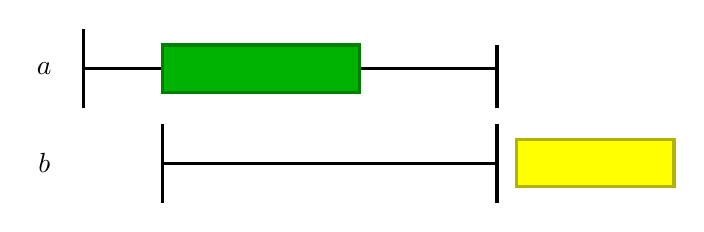
\begin{tikzpicture}
        \coordinate (A) at (0, 17mm);
        \coordinate (B) at (52.5mm, 17mm);
        \coordinate (A1) at (0, 12mm);
        \coordinate (A2) at (0, 22mm);
        \coordinate (B1) at (52.5mm, 12mm);
        \coordinate (B2) at (52.5mm, 20mm);

        \coordinate (C) at (52.5mm, 5mm);
        \coordinate (D) at (\widthpic, 5mm);
        \coordinate (C1) at (52.5mm, 0mm);
        \coordinate (C2) at (52.5mm, 10mm);
        \coordinate (D1) at (\widthpic, 0mm);
        \coordinate (D2) at (\widthpic, 10mm);

        \draw [very thick] (A) -- (B);
        \draw [very thick] (C) -- (D);

        \node at (-5mm,17mm) {$a$};
        \node at (-5mm,5mm) {$b$};

        % ergens in het midden
        \filldraw[very thick, draw=darkgreen,fill=lightgreen] (10mm, 14mm) rectangle (35mm, 20mm);
        \filldraw[very thick, draw=darkyellow,fill=lightyellow] (55mm, 2mm) rectangle (75mm, 8mm);
        
        \draw [very thick] (A1) -- (A2);
        \draw [very thick] (B1) -- (B2);
        \draw [very thick] (C1) -- (C2);
        \draw [very thick] (D1) -- (D2);
    \end{tikzpicture}
\end{frame}

\begin{frame}\frametitle{Linear Programming}
    \begin{definitie}
        \begin{align}
            \text{max:}& \quad \sum_{t \in T} (t^+ - t^-) & \nonumber \\
            \text{met voorwaarden:} & \quad 0 \leq t^+ - t^- & \forall t \in T \nonumber \\
                                    & \quad t^+ - t^- \leq c & \forall (t^+ - t^{'-} \leq c) \in C \nonumber
        \end{align}
    \end{definitie}
\end{frame}

\begin{frame}[fragile]\frametitle{Chaining}
    \begin{itemize}      
        \item Resource conflicten oplossen
    \end{itemize}
    \vspace{5mm}
    \newcommand{\widthpic}{100mm}
    \newcommand{\heightpic}{30mm}
    \newcommand\dashline[1]{\draw[thick, dashed] (0, #1) -- (100mm, #1)}
    \newcommand\normline[1]{\draw[very thick] (0, #1) -- (100mm, #1)}
    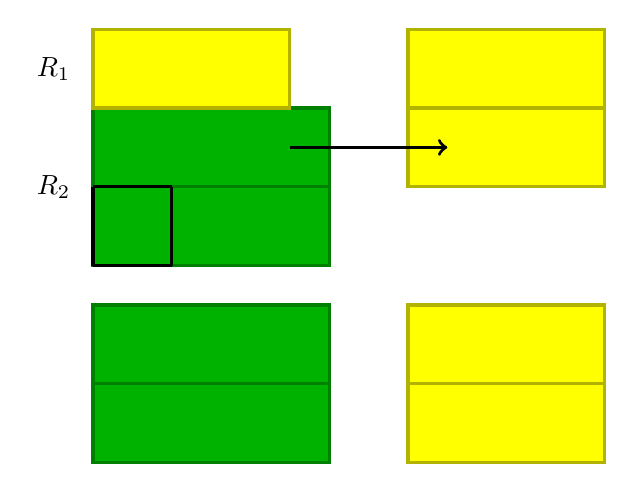
\begin{tikzpicture}
        \coordinate (A) at (0, 0);
        \coordinate (B) at (\widthpic, 0);
        \coordinate (C) at (\widthpic, \heightpic);
        \coordinate (D) at (0, \heightpic);

        % onder de resources
        % taak A
        \filldraw[very thick, draw=darkgreen,fill=lightgreen, visible on=<1>] (0mm, -15mm) rectangle (30mm, -5mm);
        \filldraw[very thick, draw=darkgreen,fill=lightgreen, visible on=<1-2>] (0mm, -25mm) rectangle (30mm, -15mm);

        % taak B
        \filldraw[very thick, draw=darkyellow,fill=lightyellow, visible on=<1-3>] (40mm, -15mm) rectangle (65mm, -5mm);
        \filldraw[very thick, draw=darkyellow,fill=lightyellow, visible on=<1-4>] (40mm, -25mm) rectangle (65mm, -15mm);
            
        % geplaatst
        % taak A
        \filldraw[very thick, draw=darkgreen,fill=lightgreen, visible on=<2->] (0mm, 10mm) rectangle (30mm, 20mm);
        \filldraw[very thick, draw=darkgreen,fill=lightgreen, visible on=<3->] (0mm, 0mm) rectangle (30mm, 10mm);

        % taak B
        \filldraw[very thick, draw=darkyellow,fill=lightyellow, visible on=<4>] (0mm, 20mm) rectangle (25mm, 30mm);
        \filldraw[very thick, draw=darkyellow,fill=lightyellow, visible on=<5->] (40mm, 20mm) rectangle (65mm, 30mm);
        \filldraw[very thick, draw=darkyellow,fill=lightyellow, visible on=<5->] (40mm, 10mm) rectangle (65mm, 20mm);

        \draw[very thick] (A) -- (B);
        \draw[very thick] (B) -- (C);
        \draw[very thick] (C) -- (D);
        \draw[very thick] (A) -- (D);

        \dashline{1 * \heightpic / 3};
        \normline{2 * \heightpic / 3};

        \node at (-5mm, 25mm) {$R_1$};
        \node at (-5mm, 10mm) {$R_2$};
        
        \draw [->, very thick, visible on=<6->] (25mm, 15mm) -- (45mm, 15mm);
    \end{tikzpicture}
\end{frame}

\input{slides/product}
\begin{frame}\frametitle{Demo}
    \huge{\hfill Tijd voor een demo! \hfill}
\end{frame}

\begin{frame}\frametitle{Software Improvement Group}
    \huge{\hfill Tijd voor SIG! \hfill}
\end{frame}

\begin{frame}\frametitle{Conclusie}
    \huge{\hfill Tijd voor een conclusie! \hfill}
\end{frame}

\begin{frame}\frametitle{Vragen}
    {\hfill%
    
\begin{tikzpicture}[thick,scale=5, every node/.style={transform shape}]
        \node at (0,0.7) {\Huge{Q}};
        \node at (0.45,0.9) {\huge{\&}};
        \node at (0.32,0.35) {\Huge{A}};
    \end{tikzpicture}%
    \hfill%
    }
\end{frame}


\end{document}
